\documentclass{ximera}
\newcommand{\RR}{\mathbb R}
\renewcommand{\d}{\,d}
\newcommand{\dd}[2][]{\frac{d #1}{d #2}}
\renewcommand{\l}{\ell}
\newcommand{\ddx}{\frac{d}{dx}}
\newcommand{\dfn}{\textbf}
\newcommand{\eval}[1]{\bigg[ #1 \bigg]}


\author{Jim Fowler and Bart Snapp}

\begin{document}

Let $F:\R^2\to\R$ be a differentiable function roughly
described by the following table of values:
\begin{image}
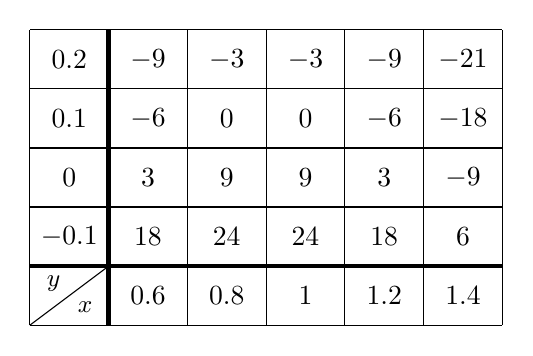
\begin{tikzpicture}[x=1cm,y=.75cm]
  \draw (0,0) grid [step=1] (6,5);
  
  \draw[ultra thick] (0,1)--(6,1);
  \draw[ultra thick] (1,0)--(1,5);
  
  \draw (0,0) -- (1,1);
  \node at (.3,.7) {\small$y$};
  \node at (0.7,.3) {\small$x$};
  
  %% y-values
  \node at (0.5,4.5) { $0.2$};
  \node at (0.5,3.5) {$ 0.1 $};
  \node at (0.5,2.5) {$ 0 $};
  \node at (0.5,1.5) {$ -0.1 $};
  
  %% x-values
  \node at (1.5,.5) {$ 0.6 $};
  \node at (2.5,.5) {$ 0.8 $};
  \node at (3.5,.5) {$ 1 $};
  \node at (4.5,.5) {$ 1.2 $};
  \node at (5.5,.5) {$ 1.4 $};
  
  %% z-values
  %% bottom row
  \node at (1.5,4.5) {$-9$};
  \node at (2.5,4.5) {$-3$};
  \node at (3.5,4.5) {$-3$};
  \node at (4.5,4.5) {$-9$};
  \node at (5.5,4.5) {$-21$};
  
  %% second row
  \node at (1.5,3.5) {$-6$};
  \node at (2.5,3.5) {$0$};
  \node at (3.5,3.5) {$0$};
  \node at (4.5,3.5) {$-6$};
  \node at (5.5,3.5) {$-18$};
  
  %% third row
  \node at (1.5,2.5) {$3$};
  \node at (2.5,2.5) {$9$};
  \node at (3.5,2.5) {$9$};
  \node at (4.5,2.5) {$3$};
  \node at (5.5,2.5) {$-9$};
  
  %% top row
  \node at (1.5,1.5) {$18$};
  \node at (2.5,1.5) {$24$};
  \node at (3.5,1.5) {$24$};
  \node at (4.5,1.5) {$18$};
  \node at (5.5,1.5) {$6$};
\end{tikzpicture}
\end{image}

\begin{problem}
What is the value of $F(1,0)$?
\begin{prompt}
\[
  F(1,0) = \answer{9}
\]
\end{prompt}

\vfill

\end{problem}

\begin{problem}
Estimate $F^{(1,0)}(1,0)$ as we did in the textbook and class.
\begin{prompt}
\[
  F^{(1,0)}(1,0) \approx \answer{-15}
\]
\end{prompt}

\vfill

\end{problem}

\begin{problem}
Estimate $F^{(0,1)}(1,0)$ as we did in the textbook and class.
\begin{prompt}
\[
  F^{(0,1)}(1,0) \approx \answer{-120}
\]
\end{prompt}

\vfill

\end{problem}


\begin{problem}
  Use your work above to give an \textbf{explicit} equation of a
  tangent plane to the graph of $F(x,y)$ at the point $(1,0)$ in terms
  of $x$ and $y$.
\begin{prompt}
\[
z = \answer{9 + (-30)(x - 1) + (-120)(y)}
\]
\end{prompt}

\vfill

\end{problem}

%%%%%%%%%%%%%%%%%%%%%%%%%%%%%%%%%%%%%%%%%%%
%%%%%%%%%%%%%%%%%%%%%%%%%%%%%%%%%%%%%%%%%%%
%% Chain Rule
%%%%%%%%%%%%%%%%%%%%%%%%%%%%%%%%%%%%%%%%%%%
%%%%%%%%%%%%%%%%%%%%%%%%%%%%%%%%%%%%%%%%%%%

\begin{problem}
  Let $\vecl(t)$ be the vector-valued function describing the line
  starting at the point $(2,-1)$ that passes through $(0,1)$ as $t$
  runs from $0$ to $1$.  Use your work above to estimate
  $\dd{t}F(\vecl(t))$ at $t = 1/2$.
  \begin{prompt}
  \[
  \eval{\dd{t} F(\vecl(t))}_{t=1/2} \approx \answer{-180}
  \]
  \end{prompt}

  \vfill
  
\end{problem}


\end{document}
